%%%%%%%%%%%%%%%%%%%%%%%%%%%%%%%%%%%%%%%%%
% Arsclassica Article
% LaTeX Template
% Version 1.1 (10/6/14)
%
% This template has been downloaded from:
% http://www.LaTeXTemplates.com
%
% Original author:
% Lorenzo Pantieri (http://www.lorenzopantieri.net) with extensive modifications by:
% Vel (vel@latextemplates.com)
%
% License:
% CC BY-NC-SA 3.0 (http://creativecommons.org/licenses/by-nc-sa/3.0/)
%
%%%%%%%%%%%%%%%%%%%%%%%%%%%%%%%%%%%%%%%%%

%----------------------------------------------------------------------------------------
%	PACKAGES AND OTHER DOCUMENT CONFIGURATIONS
%----------------------------------------------------------------------------------------

\documentclass[
10pt, % Main document font size
a4paper, % Paper type, use 'letterpaper' for US Letter paper
oneside, % One page layout (no page indentation)
%twoside, % Two page layout (page indentation for binding and different headers)
headinclude,footinclude, % Extra spacing for the header and footer
BCOR5mm, % Binding correction
]{scrartcl}

%%%%%%%%%%%%%%%%%%%%%%%%%%%%%%%%%%%%%%%%%
% Arsclassica Article
% Structure Specification File
%
% This file has been downloaded from:
% http://www.LaTeXTemplates.com
%
% Original author:
% Lorenzo Pantieri (http://www.lorenzopantieri.net) with extensive modifications by:
% Vel (vel@latextemplates.com)
%
% License:
% CC BY-NC-SA 3.0 (http://creativecommons.org/licenses/by-nc-sa/3.0/)
%
%%%%%%%%%%%%%%%%%%%%%%%%%%%%%%%%%%%%%%%%%

%----------------------------------------------------------------------------------------
%	REQUIRED PACKAGES
%----------------------------------------------------------------------------------------

\usepackage[
nochapters, % Turn off chapters since this is an article        
beramono, % Use the Bera Mono font for monospaced text (\texttt)
eulermath,% Use the Euler font for mathematics
pdfspacing, % Makes use of pdftex’ letter spacing capabilities via the microtype package
dottedtoc % Dotted lines leading to the page numbers in the table of contents
]{classicthesis} % The layout is based on the Classic Thesis style

\usepackage{arsclassica} % Modifies the Classic Thesis package

\usepackage[T1]{fontenc} % Use 8-bit encoding that has 256 glyphs

\usepackage[utf8]{inputenc} % Required for including letters with accents

\usepackage{graphicx} % Required for including images
\graphicspath{{Figures/}} % Set the default folder for images

\usepackage{enumitem} % Required for manipulating the whitespace between and within lists

\usepackage{lipsum} % Used for inserting dummy 'Lorem ipsum' text into the template

\usepackage{subfig} % Required for creating figures with multiple parts (subfigures)

\usepackage{amsmath,amssymb,amsthm} % For including math equations, theorems, symbols, etc

\usepackage{varioref} % More descriptive referencing

%----------------------------------------------------------------------------------------
%	THEOREM STYLES
%---------------------------------------------------------------------------------------

\theoremstyle{definition} % Define theorem styles here based on the definition style (used for definitions and examples)
\newtheorem{definition}{Definition}

\theoremstyle{plain} % Define theorem styles here based on the plain style (used for theorems, lemmas, propositions)
\newtheorem{theorem}{Theorem}

\theoremstyle{remark} % Define theorem styles here based on the remark style (used for remarks and notes)

%----------------------------------------------------------------------------------------
%	HYPERLINKS
%---------------------------------------------------------------------------------------

\hypersetup{
%draft, % Uncomment to remove all links (useful for printing in black and white)
colorlinks=true, breaklinks=true, bookmarks=true,bookmarksnumbered,
urlcolor=webbrown, linkcolor=RoyalBlue, citecolor=webgreen, % Link colors
pdftitle={}, % PDF title
pdfauthor={\textcopyright}, % PDF Author
pdfsubject={}, % PDF Subject
pdfkeywords={}, % PDF Keywords
pdfcreator={pdfLaTeX}, % PDF Creator
pdfproducer={LaTeX with hyperref and ClassicThesis} % PDF producer
} % Include the structure.tex file which specified the document structure and layout

\hyphenation{Fortran hy-phen-ation} % Specify custom hyphenation points in words with dashes where you would like hyphenation to occur, or alternatively, don't put any dashes in a word to stop hyphenation altogether
\usepackage{float}
%----------------------------------------------------------------------------------------
%	TITLE AND AUTHOR(S)
%----------------------------------------------------------------------------------------

\title{Dispersed two phase flow in sudden expansion pipe} % The article title

\author{\spacedlowsmallcaps{Yapi Donatien Achou}} % The article author(s) - author affiliations need to be specified in the AUTHOR AFFILIATIONS block

\date{} % An optional date to appear under the author(s)

%----------------------------------------------------------------------------------------

\begin{document}

%----------------------------------------------------------------------------------------
%	HEADERS
%----------------------------------------------------------------------------------------

\renewcommand{\sectionmark}[1]{\markright{\spacedlowsmallcaps{#1}}} % The header for all pages (oneside) or for even pages (twoside)
%\renewcommand{\subsectionmark}[1]{\markright{\thesubsection~#1}} % Uncomment when using the twoside option - this modifies the header on odd pages
\lehead{\mbox{\llap{\small\thepage\kern1em\color{halfgray} \vline}\color{halfgray}\hspace{0.5em}\rightmark\hfil}} % The header style

\pagestyle{scrheadings} % Enable the headers specified in this block

%----------------------------------------------------------------------------------------
%	TABLE OF CONTENTS & LISTS OF FIGURES AND TABLES
%----------------------------------------------------------------------------------------

\maketitle % Print the title/author/date block

\setcounter{tocdepth}{2} % Set the depth of the table of contents to show sections and subsections only

\tableofcontents % Print the table of contents

\listoffigures % Print the list of figures

\listoftables % Print the list of tables



\section{Introduction}
Disperse two-phase flows is the flow regime in which one phase is dispersed in the other phase called continuous phase. Example of disperse flows are gas-solid, gas-liquid, liquid-liquid, solid-gas. In gas-solid the disperse phase is always in solid phase because solid particle never coalesce with each other. In gas-liquid flows the dispersed phase is determined mainly by the flow rate of both phases because the interface between both phases is deformable. An increased in the mass flow rate create coalescence between the disperse phase elements and the disperse phase becomes the continuous phase. This phase interaction between dispersed and continuous phase demonstrate a dynamic change in the topology of the phases in presence. Therefore the mathematical model describing two-phase disperse flows must incorporate this phase interaction.

\section{Mathematical model}
The mathematical model describing two-phase disperse flows used in this project is based on an Eulerian two fluids approach presented in \cite{behzadi:2003}. In the Eulerian approach the Eulerian conservation equations are used to describe both the dispersed and the continuous phase in a fixed coordinate system \cite{Hill:1998}. The two fluid equations are derived from the conservation of mass, momentum and energy by applying suitable averaging procedure. The model derived in \cite{behzadi:2003} uses ensemble averaging. The ensemble average of a scalar or vector field $\phi$ is given by
\begin{equation}
\bar{\phi} = \frac{1}{N}\sum_{j=1}^{N}{\phi_{j}} \nonumber
\end{equation}
where $N$ is the total number of realisation in the ensemble and $\phi_{j}$ is the value of $\phi$
for the realisation $j$. The derivation of the model equations is based on  the phase-weighted two-fluid model introduced in \cite{Ishii:1975}. The phase-weighted mean of $\phi$ is $\tilde{\phi}$ with 
\begin{equation}
\phi = \tilde{\phi}+\phi^{\prime\prime}\nonumber
\end{equation}

\begin{equation}
\tilde{\phi} = \frac{\overline{\alpha\phi}}{\bar{\alpha}}\nonumber
\end{equation}
where $\phi^{\prime\prime}$ is a fluctuation component and $alpha$ is the phase fraction. Using this ensemble averaging, the continuity and momentum equation respectively given by

\begin{equation}
\frac{\partial \bar{\alpha_{i}}}{\partial t}+\nabla\cdot(\tilde{\textbf{u}}_{i}\bar{\alpha_{i}}) = 0
\end{equation}

\begin{equation}
\frac{\partial \bar{\alpha_{i}} \tilde{\textbf{u}}_{i}}{\partial t}+\nabla\cdot(\bar{\alpha}_{i}\tilde{\textbf{u}}_{i}\tilde{\textbf{u}}_{i})+\nabla\cdot(\bar{\alpha}_{i}
\textbf{R}_{i}) =-\frac{\bar{\alpha}_{i}}{\rho_{i}}\nabla\bar{p}+\bar{\alpha}_{i}\textbf{g}+
\frac{\bar{\textbf{M}}_{i}}{\rho_{i}}
\end{equation}
where $\tilde{\textbf{u}}_{i}$ is the weighted-mean velocity of phase $i = d,c$ where $d$ stand for disperse phase and $c$ stand for continuous phase. $\rho$, $\bar{p}$ are the fluid density and ensemble average pressure respectively. $\textbf{R}$ and $\bar{\textbf{M}}$ are the Reynold stress and the ensemble average of the inter-facial momentum transfer term fully described in \cite{behzadi:2003}. 

\subsection{Turbulence model}
The mixture $k-\epsilon$ model takes in to account the dynamics occurring between the phases. In preview models turbulence was dominated by the continuous phase. These modeled are only valid for dilute systems in which the disperse phase elements (particles, bubble, droplet) interation are neglected. For high phase fraction interaction of disperse phase element occur.In the turbulent model given in \cite{behzadi:2003} and used in this project the two fluids are regarded as one fluid with new properties, such as mixture density, mixture kinetic energy, mixture rate of dissipation, expressed in terms of the properties of the continuous phase and the disperse phase. The turbulence model is given by

\begin{equation}
\frac{\partial (\rho_{m}k_{m})}{\partial t}+\nabla\cdot(\rho_{m}\tilde{\textbf{u}}_{m}k_{m})=
\nabla\cdot\left(\frac{\mu_{m}^{t}}{\sigma_{m}}\right)\nabla k_{m} +P_{k}^{m}-\rho_{m}\epsilon_{m}+S_{k}^{m}
\end{equation}
\begin{equation}
\frac{\partial (\rho_{m}\epsilon_{m})}{\partial t}+\nabla\cdot(\rho_{m}\tilde{\textbf{u}}_{m}\epsilon_{m})=
\nabla\cdot\left(\frac{\mu_{m}^{t}}{\sigma_{m}}\right)\nabla \epsilon_{m} +\left(\frac{\epsilon_{m}}{k_{m}}\right)(C_{\epsilon 1}P_{k}^{m}-C_{\epsilon 2\rho_{m}\epsilon_{m}})+C_{\epsilon 3}\left(\frac{\epsilon_{m}}{k_{m}}\right) S_{k}^{m}
\end{equation}
the suffix $m$ denote mixture of the two phases. The mixture phase can be related to the continuous phase as followed \cite{behzadi:2003}:

\begin{equation}
k_{d} = C_{t}^{2}k_{c} \nonumber
\end{equation}

\begin{equation}
\epsilon_{d} = C_{t}^{2}\epsilon_{c} \nonumber
\end{equation}

\begin{equation}
\rho_{m}= \bar{\alpha}_{c}\rho_{c}+\bar{\alpha}_{d}\rho_{d} \nonumber
\end{equation}

\begin{equation}
k_{m} = \left(  \bar{\alpha}_{c} \frac{\rho_{c}}{\rho_{m}}+ \bar{\alpha}_{d}\frac{\rho_{d}}{rho_{m}}C_{t}^{2}   \right)k_{c} \nonumber
\end{equation}

\begin{equation}
\epsilon_{m} = \left(  \bar{\alpha}_{c} \frac{\rho_{c}}{\rho_{m}}+ \bar{\alpha}_{d}\frac{\rho_{d}}{rho_{m}}C_{t}^{2}   \right)\epsilon_{c} \nonumber
\end{equation}

The rest of the mixture properties are fully described in \cite{behzadi:2003}

\section{Numerical treatment}
The flow is solve for pressure $p$, velocity $u$ and kinetic energy $k$ and rate of dissipation $\epsilon$ using EulertwophaseFoam solver. The domain is a sudden expansion vertical pipe see figure 1


\begin{figure}[H]
  \caption{Computational domain}
  \centering
    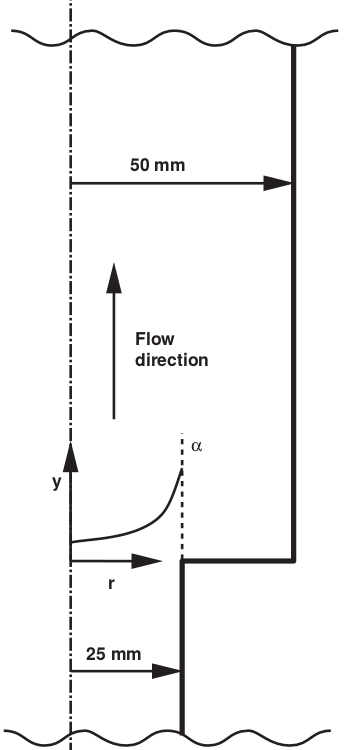
\includegraphics[width=0.3\textwidth]{pipe.png}
\end{figure}

The mean liquid velocity at the inlet is $u_{l} =1.57$ and the relative velocity of the phases is $u_{l}-u_{g} = 0.3$. The flow is two dimensional axisymmetric and steady.

\section{Project progression}
In the first phase of the project a laminar two phase will be simulated. If convergence is reach the complexity of the flow will be extended to a turbulent two-phase disperse flow.
%----------------------------------------------------------------------------------------
%	BIBLIOGRAPHY
%----------------------------------------------------------------------------------------

\renewcommand{\refname}{\spacedlowsmallcaps{References}} % For modifying the bibliography heading

\bibliographystyle{unsrt}

\bibliography{sample.bib} % The file containing the bibliography

%----------------------------------------------------------------------------------------

\end{document}